% ----------------------------------------
% ----------------------------------------
% Šablon za prezentaciju
% Autor: Miloš D. Petrašinović <mpetrasinovic@mas.bg.ac.rs>
% Masinski fakultet, Univerzitet u Beogradu
% Katedra za vazduhoplovstvo, Struktura letelica
% https://vazmfb.com
% Beograd, 2023
% ----------------------------------------
% ----------------------------------------

% ----------------------------------------
% Definisanje korišćenih paketa i formata rada
% ----------------------------------------
\documentclass[12pt]{beamer}
\usetheme{_vazmfb}
\usepackage[T1]{fontenc}
\usepackage[utf8]{inputenc}
\usepackage{tikz}
\usepackage{ulem}
\usepackage{lineno}
\usepackage{hyperref}
\usepackage{subcaption}
\usepackage{textcomp}
\usepackage{setspace}
\usepackage{gensymb}
\usepackage[numbered]{matlab-prettifier}
\usepackage{graphicx}
\usepackage[english]{babel}
\usepackage{placeins}
\usepackage{amssymb}
\usepackage{amsmath}
\usepackage[toc,title]{appendix}
\usepackage{nomencl}
\usepackage{float}
\usepackage[figurename=Slika, tablename=Tabela]{caption}
\usepackage{bigstrut}
\usepackage{booktabs}
\usepackage{colortbl}
\usepackage{multirow}
\usepackage{multicol}
\usepackage{siunitx}
\usepackage{array}
\usepackage{fancyvrb}
\usepackage{icomma}
\usepackage{lmodern}
\usepackage{listings}
\usepackage{diagbox}
\usepackage{bm}
\usepackage[numbered]{matlab-prettifier}

% Folder za slike
\graphicspath{{slike/}}

% Boje
\definecolor{tamno-plava}{cmyk}{1,0.79,0.32,0.17}
\definecolor{svetlo-plava}{cmyk}{0.93,0.64,0.03,0}
\definecolor{siva}{cmyk}{0.73,0.67,0.65,0.8}
\definecolor{tamno-siva}{HTML}{aaaaaa}
\definecolor{zelena}{cmyk}{1,0,1,0.5}

% Nabrajanje
\newcommand\itemS{\item[\textbf{\S}]}

% Matrice 
\makeatletter
\renewcommand*\env@matrix[1][c]{\hskip -\arraycolsep
  \let\@ifnextchar\new@ifnextchar
  \array{*\c@MaxMatrixCols #1}}
\makeatother

% Matlab kod
\lstset{
  style = Matlab-editor,
  basicstyle = \fontfamily{pcr}\selectfont\footnotesize, % if you want to use Courier
  numberstyle = \tiny\color{siva},
  commentstyle = \color{zelena},
}

% Merne jedinice
\sisetup{
  per-mode=fraction,
  fraction-function=\tfrac
}

% Norme
\newcommand{\norm}[1]{\left\lVert#1\right\rVert}
\newcommand{\abs}[1]{\left\lvert#1\right\rvert}
\newcommand{\diff}[1]{\mathrm{d}#1}

% Font
\usefonttheme{default}
%\usefonttheme{serif}

% Bez nastavljanja u sledecem redu
\tolerance=1
\emergencystretch=\maxdimen
\hyphenpenalty=10000
\hbadness=10000

%----------------------------------
% Podaci
%----------------------------------

\title[Naziv predmeta]{Naziv predmeta} % Uneti naziv predmeta
\subtitle{Naslov prezentacije} % Uneti naslov prezentacije
\date{20.11.2023.} % Uneti datum prezentacije
\institute[Katedra za vazduhoplovstvo]{\textbf{Katedra za vazduhoplovstvo} \\ Mašinski fakultet \\ Univerziteta u Beogradu}
\authorsgroup{\orcid{Ime Prezime}{0000-0000-0000-0000}} % Zameniti ime i prezime ali i 0000-0000-0000-0000 sa ORCID
\webpage{vazmfb.com/predmet/} % Zameniti predmet sa adresom predmeta
\webpageurl{https://vazmfb.com/predmet/} % Zameniti predmet sa adresom predmeta

% ----------------------------------------
% POCETAK DOKUMENTA
% ----------------------------------------
\begin{document}

% ----------------------------------------
% PRVI FRAME
% ----------------------------------------
{
	\setbeamertemplate{headline}{}
	\setbeamertemplate{footline}{}
	\maketitle
}
\addtocounter{framenumber}{-1} % bez brojanja prve strane

% ----------------------------------------
% Section
% ----------------------------------------
\section{Naslov sekcije}

% ----------------------------------------
% FRAME
% ----------------------------------------
\begin{frame}{Naslov slajda}

Ubacivanje slike (slika \ref{orao}) u prezentaciju % Referenciranje sa \label i \ref

\begin{figure}
    \centering
    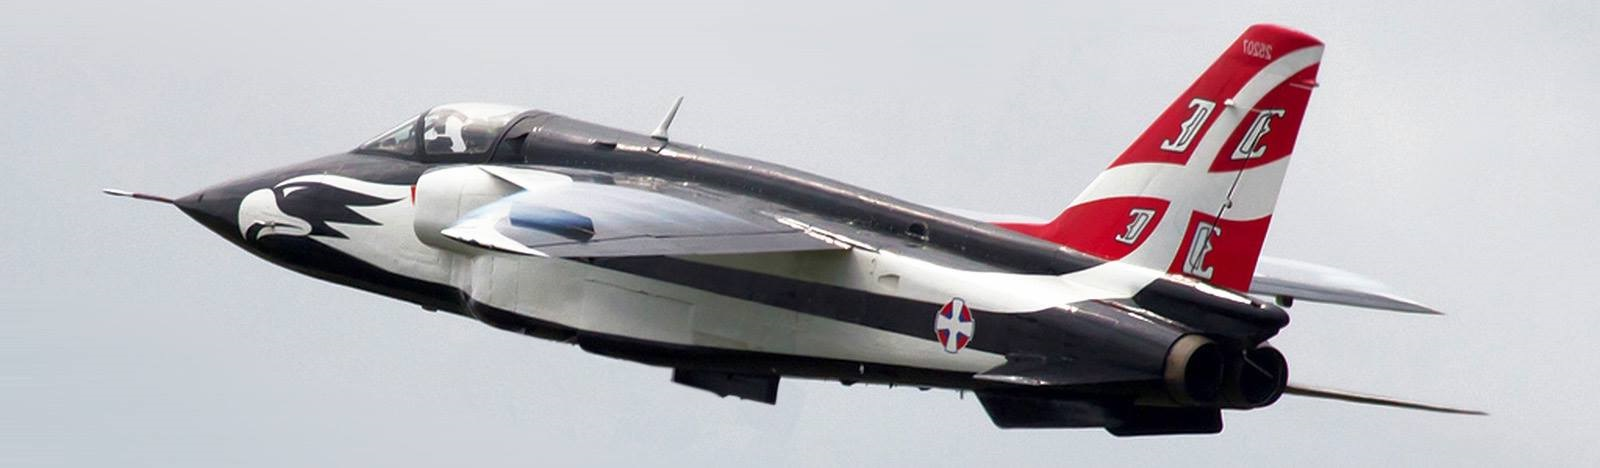
\includegraphics[width=0.9\textwidth]{orao}
    \caption{Naslov slike}
    \label{orao}
\end{figure}
\end{frame}

% ----------------------------------------
% FRAME
% ----------------------------------------
\begin{frame}{}
Liste i podela slajda na dva dela

\vspace{1cm} % vertikalno rastojanje

% Leva polovina
\begin{minipage}{0.49\textwidth}
    \begin{itemize}
    	\item Prvi 
    	\item Drugi
    	\item Treci
    \end{itemize}
\end{minipage}
% Desna polovina
\begin{minipage}{0.49\textwidth}
    \begin{enumerate}
    	\item Prvi 
    	\item Drugi
    	\item Treci
    \end{enumerate}
\end{minipage}

\vspace{1cm} % vertikalno rastojanje

\textit{Adresa internet stranice sa linkom:} % Italic tekst
\url{https://vazmfb.com}

\href{https://vazmfb.com}{Tekst sa linkom ka vazmfb.com}

\end{frame}

% ----------------------------------------
% FRAME
% ----------------------------------------
\begin{frame}{Novi naslov slajda}
\begin{vazmfb_block}{Naslov definicije}
    Tekst definicije
\end{vazmfb_block}

Jednačina \ref{eq1} % Na isti način se vrši referenciranje i jednacina i svih ostalih elemenata
\begin{equation}
    \label{eq1}
    \Pi = \frac{1}{2} \int_{V} \bm{\varepsilon}^T\, \bm{\sigma}\, \text{d}V = \frac{1}{2} \int_{V} \bm{\varepsilon}^T\, \bm{c}\, \bm{\varepsilon}\, \diff{V}
\end{equation}

\end{frame}

% ----------------------------------------
% FRAME
% ----------------------------------------
\begin{frame}{}


Program primer:
\lstinputlisting[language=Matlab, caption=Naslov programa]{programi/program.m}

Primer \textbf{matrične jednačine} % Bold tekst
\footnotesize
\begin{equation}
    \begin{bmatrix}
       \sigma_{xx} \\
       \sigma_{yy} \\
       \sigma_{zz} \\
       \sigma_{yz} \\
       \sigma_{xz} \\
       \sigma_{xy} \\
    \end{bmatrix} 
     = 
    \begin{bmatrix}
       c_{11} & c_{12} & c_{13} & c_{14} & c_{15} & c_{16} \\
       & c_{22} & c_{23} & c_{24} & c_{25} & c_{26} \\
       & & c_{33} & c_{34} & c_{35} & c_{36} \\
       & & & c_{44} & c_{45} & c_{46} \\
       & & & & c_{55} & c_{56} \\
       \multicolumn{2}{c}{\text{Sim.}} & & & & c_{66} \\
    \end{bmatrix} 
    \begin{bmatrix}
       \varepsilon_{xx} \\
       \varepsilon_{yy} \\
       \varepsilon_{zz} \\
       \gamma_{yz} \\
       \gamma_{xz} \\
       \gamma_{xy} \\
    \end{bmatrix} 
\end{equation}

\end{frame}

% ----------------------------------------
% FRAME
% ----------------------------------------
\begin{frame}{}

Primer tabele

\begin{table}[H]
\large
\centering
\caption{Naslov tabele}
\begin{tabular}[H]{|l|c|}
\hline
Prva ćelija & Desno \\ \hline
Dole & Dijagonala \\ \hline
\end{tabular}
\end{table}
\end{frame}

\section{Kraj prezentacije}
% ----------------------------------------
% FRAME
% ----------------------------------------
\begin{frame}
\centering
\Huge Hvala na pažnji!
\end{frame}

% ----------------------------------------
% KRAJ DOKUMENTA
% ----------------------------------------
\end{document}
